Within micrometer wavelengths, photonic crystals and gratings can be used to guide or diffract electromagnetic waves, while similar X-ray manipulations can use crystals with atoms regularly spaced a few nanometers apart, as scattering centers. At the same time, a large gap between these wavelength ranges, called XUV (extreme-ultraviolet) or hard ultraviolet, turns out to be difficult to manipulate. To solve this problem, we propose the use of arrays of spherical nanoclusters for directed scattering of hard ultraviolet radiation (Fig.~\ref{intsch:image}).

\begin{tikzfigure}
    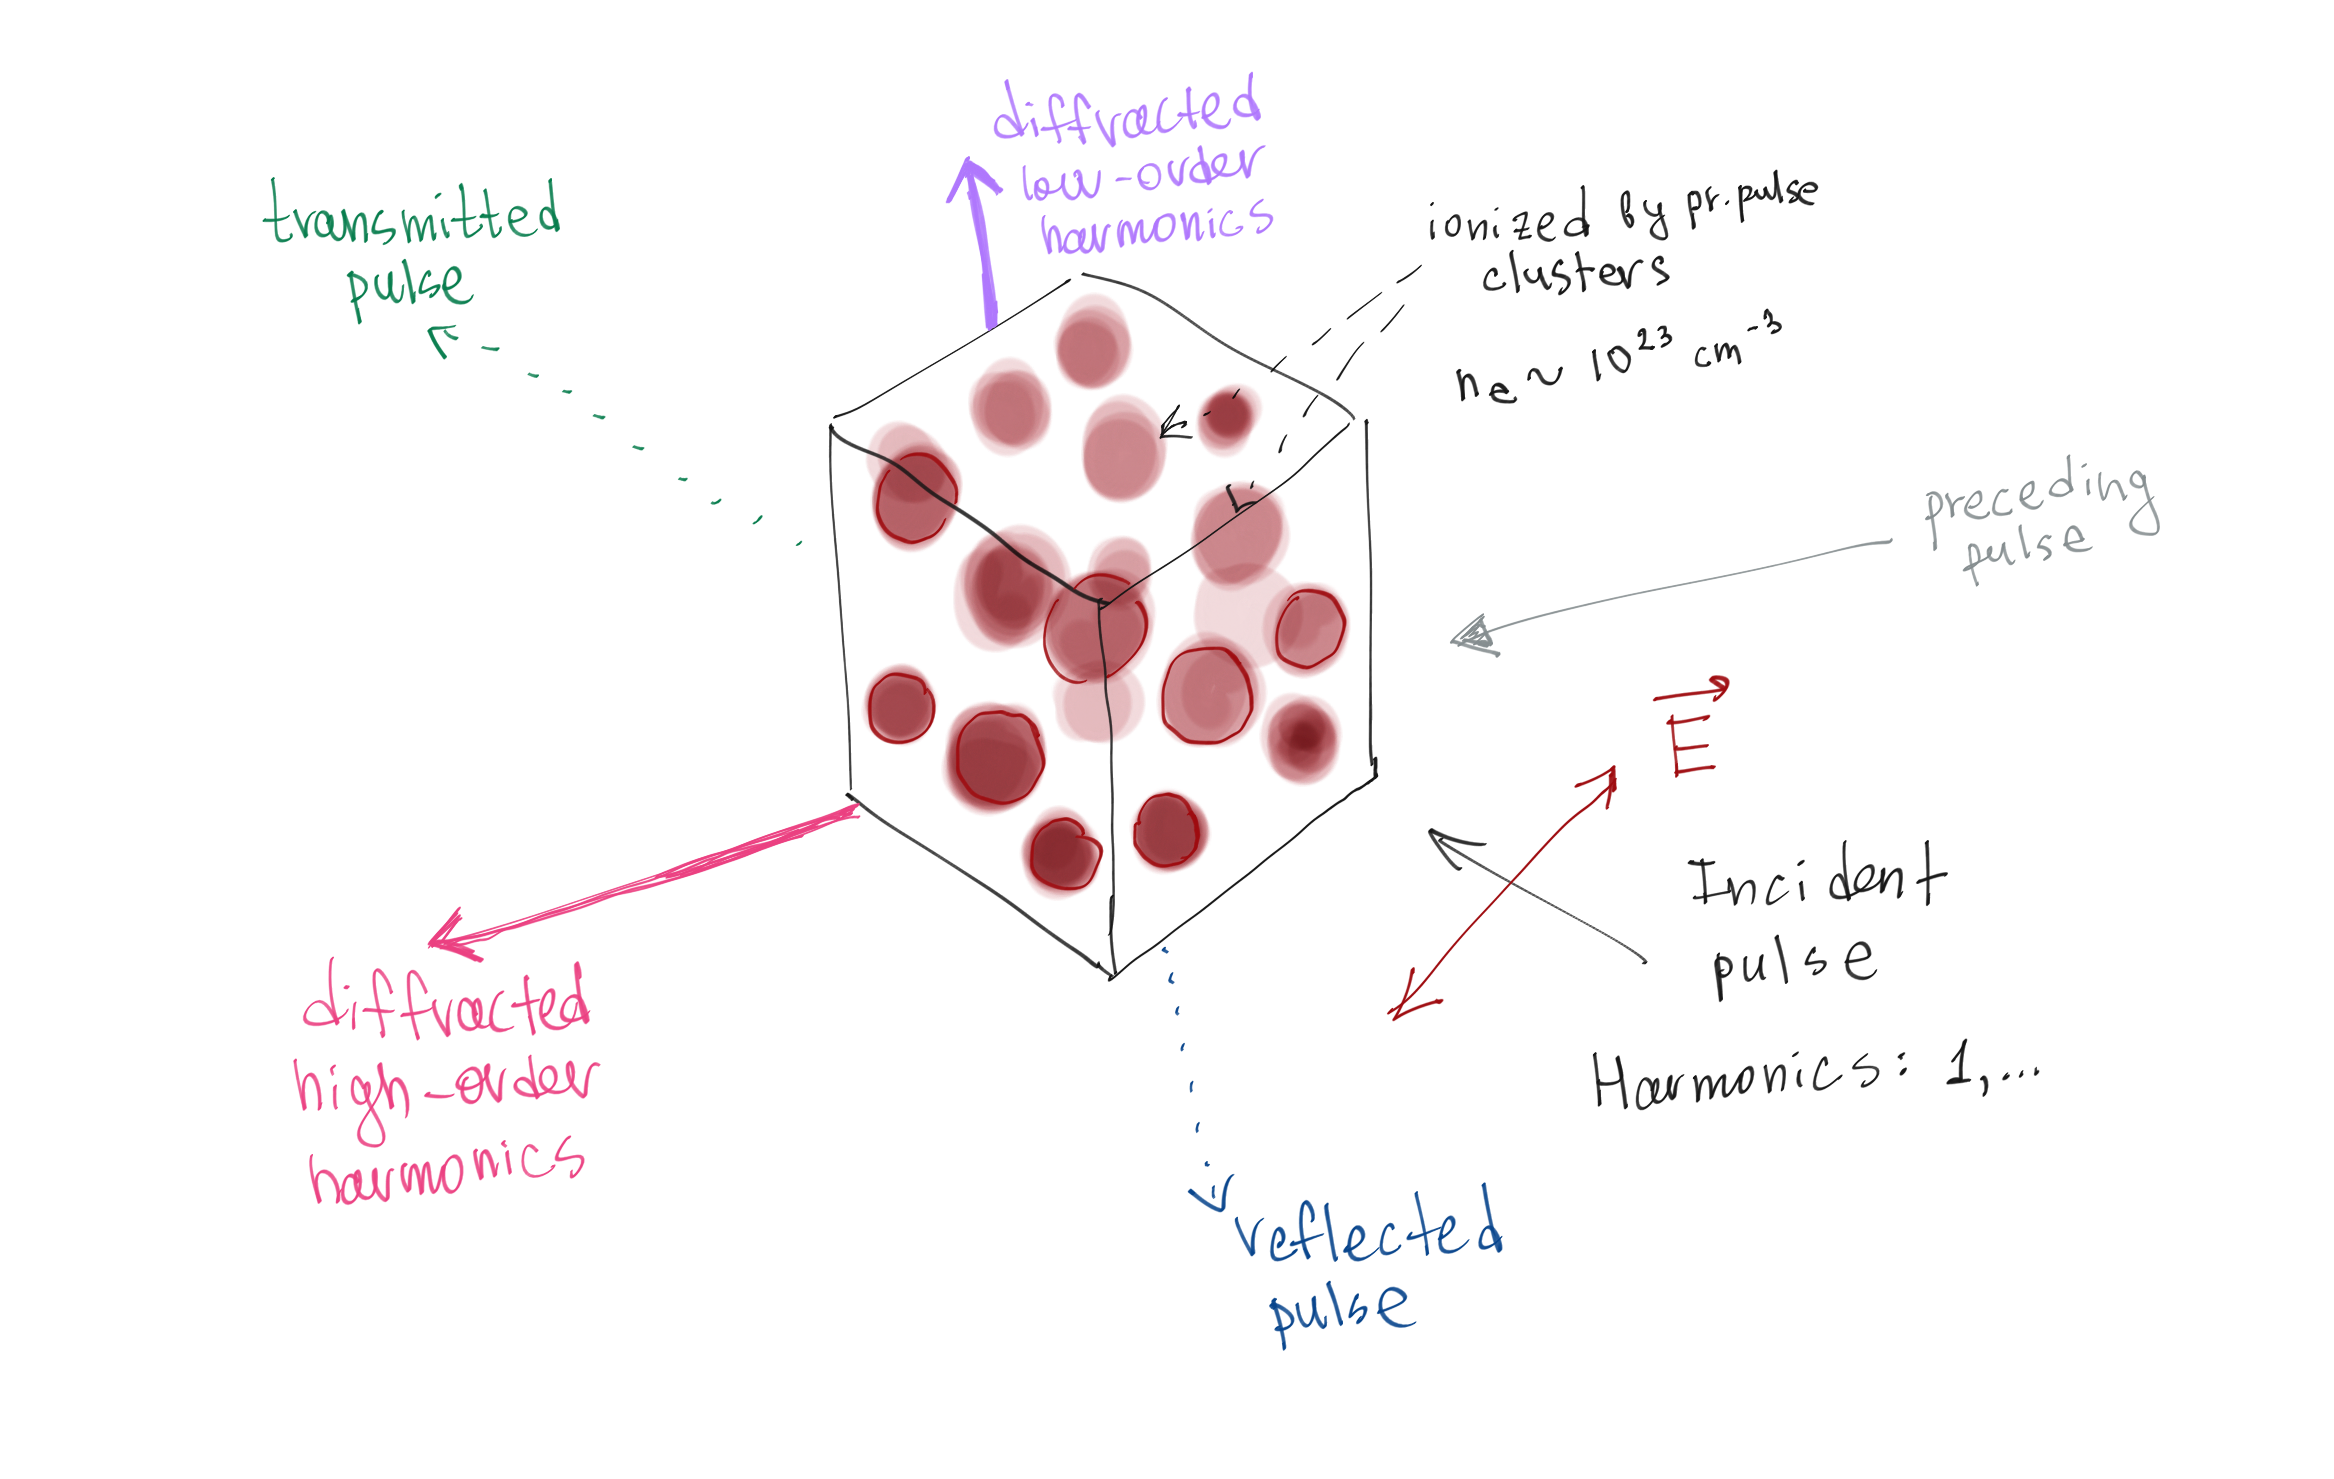
\includegraphics[width=0.83\linewidth]{../img/plasma_area2}\label{intsch:image}\caption{An interaction scheme. The plane of polarization is parallel to one of the faces of the cubic region. The sizes of spherical clusters are on the order of a few nanometers, and the distance between them is at least hundreds of nanometers. The distribution of clusters inside the cubic region is generally arbitrary.}
\end{tikzfigure}